\documentclass[12pt]{article}
\usepackage{geometry}
\geometry{a4paper, margin=1in}
\usepackage[utf8]{inputenc}
\usepackage[T1]{fontenc}
\usepackage{parskip}
\usepackage{graphicx}
\usepackage{caption}
\usepackage{tabularx}
\usepackage{float}
\usepackage{fancyhdr}

\geometry{
 a4paper,
 total={170mm,257mm},
 left=20mm,
 top=20mm,
}

\setlength{\headheight}{15pt} % Sets the height of the header

\pagestyle{empty} % No headers or footers for other pages
\fancypagestyle{firstpage}{ % Custom header for the first page
 \lhead{3 Giugno 2023}
 \rhead{Marcello Ferrara}
 \renewcommand{\headrulewidth}{0pt}
}

\begin{document}

\thispagestyle{firstpage} % Apply the custom first page style

\begin{center}
    
\includegraphics[width=0.20\textwidth]{logo.png} \\[1cm] % Logo
    \Large\textbf{Relazione di Laboratorio: Oscillazioni Forzate e Smorzate in un Sistema Massa-Molla} \\ % Title
\end{center}

\vspace*{1cm} % Adds vertical space after the title

\begin{abstract}
Questo studio esamina il fenomeno della risonanza in un sistema massa-molla sottoposto a oscillazioni forzate e smorzate. L'obiettivo principale è stato quello di osservare il comportamento del sistema quando è soggetto a una forza esterna periodica, con particolare attenzione al fenomeno della risonanza. Il valore sperimentale ottenuto per la frequenza di risonanza è risultato in accordo con le aspettative teoriche. La curva di risonanza sperimentale è stata confrontata con la curva teorica, e la compatibilità tra le due è stata quantificata attraverso il test del chi quadro, risultando in una probabilità di compatibilità del 99,4\%. Questi risultati confermano la validità del modello teorico utilizzato per descrivere il comportamento del sistema.
\end{abstract}

% =================================================================================================

\section{Introduzione}

L'obiettivo di questa relazione è esaminare il fenomeno della risonanza in un sistema massa-molla sottoposto a oscillazioni forzate e smorzate. Il sistema massa-molla è un modello fisico fondamentale, utilizzato per descrivere una vasta gamma di fenomeni oscillatori. Questo sistema è governato dalla legge di Hooke, che afferma che la forza esercitata dalla molla è proporzionale allo spostamento della massa dalla sua posizione di equilibrio.

Il fenomeno di risonanza si verifica quando la frequenza della forza esterna applicata al sistema coincide con la frequenza naturale del sistema, portando a un aumento significativo dell'ampiezza delle oscillazioni. In questo esperimento, siamo interessati a osservare e analizzare la curva di risonanza, nota come curva "Lorentziana", e a confrontare i risultati sperimentali con le previsioni teoriche.

Abbiamo misurato l'ampiezza di oscillazione per diverse frequenze/pulsazioni in un intorno della condizione di risonanza e costruito la curva Lorentziana sperimentale. Abbiamo anche costruito la curva Lorentziana attesa e verificato l'accordo tra le due curve. Come bonus, abbiamo osservato il fenomeno dei battimenti.

Un aspetto di questo esperimento riguarda la gestione delle incertezze. Durante la raccolta dei dati, l'analisi e l'interpretazione dei risultati, le incertezze sono state stimate e propagate. Per minimizzare l'incertezza, abbiamo adottato una serie di procedure. Queste includono l'uso di strumenti calibrati, la ripetizione delle misurazioni per mitigare l'errore casuale e l'applicazione di tecniche statistiche appropriate per l'analisi dei dati. Questo approccio ha contribuito a ridurre l'incertezza associata ai risultati ottenuti.

% =================================================================================================

\section{Modello Teorico}

Il modello teorico utilizzato per questo esperimento è il sistema massa-molla smorzato e forzato. Questo sistema è descritto da una serie di equazioni che rappresentano diversi aspetti del suo comportamento.

Il moto del sistema in assenza di forzante esterna è governato dal moto armonico smorzato, che tiene conto dell'attrito presente nel sistema:

\[
  {\frac{\mathrm{d^2}x(t)}{\mathrm{d}t^2}}=-\omega_0^2x(t)-2\gamma\frac{\mathrm{d} x}{\mathrm{d}t}
\]

dove $x$ è lo spostamento dalla posizione di equilibrio.

La pulsazione propria dell'oscillatore $\omega_0$ rappresenta la frequenza naturale del sistema, ovvero la frequenza alla quale il sistema oscilla in assenza di forzante esterna e smorzamento.

\[
  \omega_0^2=\frac{k}{m}
\]

dove $k$ è la costante elastica della molla e $m$ la massa.

Il termine di smorzamento descrive l'effetto dell'attrito sul sistema, che tende a ridurre l'ampiezza delle oscillazioni nel tempo. Il termine di smorzamento è:

\[
  2\gamma=\frac{C_1}{m}
\]

dove $C_1$ è il coefficiente che determina la forza dello smorzamento proporzionale alla velocità.

Quando il sistema è soggetto a una forza esterna periodica, il suo comportamento cambia ed è descritto dal moto armonico smorzato e forzato, in cui il termine aggiuntivo descrive l'effetto della forza:

\[
  {\frac{\mathrm{d^2}x(t)}{\mathrm{d}t^2}}=-\omega_0^2x(t)-2\gamma\frac{\mathrm{d} x}{\mathrm{d}t}+\frac{F_0}{m}e^{i\omega_ft}
\]

dove $F_0$ è la forza esterna massima e $\omega_f$ la frequenza della forzante.

La soluzione dell'equazione del moto permette di determinare l'ampiezza massima delle oscillazioni in funzione della frequenza forzante:

\[
  A(\omega_f)=\frac{F_0}{m\sqrt{\bigg(\omega_0^2-\omega_f^2\bigg)^2+4\gamma^2\omega_f^2}}
\]

La funzione descrive quindi una Lorentziana.

Nella nostra analisi, prenderemo in considerazione tre proprietà fondamentali della curva Lorentziana, dato che queste forniscono informazioni sul comportamento del sistema in risonanza.
Il centroide della curva che coincide con $\omega_0$, il valore del massimo $A_{max}$ e la larghezza a metà altezza (FWHM) denotata con $\Delta \omega$.
\[
  A_{max}=\frac{F_0}{2\omega_0m\gamma} \qquad \Delta \omega=2\sqrt3\gamma
\]

Per quanto riguarda le non idealità del modello, ci sono diverse fonti di attrito non ideali che possono influenzare il comportamento del sistema. Ad esempio, l'attrito può essere proporzionale alla velocità al quadrato, piuttosto che alla velocità. Questo tipo di attrito non ideale è stato minimizzato sperimentalmente con i dati dell'esperienza precedente. Inoltre, l'energia può essere sottratta dal sistema a causa della deformazione della molla o perché il sistema non oscilla in modo perfettamente verticale.
Infine va notato che è solo grazie allo smorzamento che la curva non diverge in $\omega_0$.
% =================================================================================================

\section{Apparato Sperimentale}

L'apparato sperimentale per il presente esperimento si compone di diversi elementi. In primo luogo, si fa riferimento a una molla di massa pari a 22,45 g, fissa solo nel suo estremo superiore, alla quale è attaccata una massa di 169,77 g in grado di oscillare liberamente lungo la direzione verticale.

Per la misurazione della posizione della massa nel tempo è impiegato un sensore di posizione di tipo sonar, situato direttamente sotto la massa stessa. Tale sensore presenta una sensibilità di 0,15 m, una risoluzione di 0,001 m e una portata di 8 m.

Nell'apparato è presente un attuatore che applica una forza esterna periodica alla massa. L'attuatore, un motore elettrico, si muove avanti e indietro simulando la forma del segnale elettrico. Ampiezza e frequenza della forza applicata sono variabili.

Una bilancia di precisione, con una sensibilità di 10 g, una risoluzione di 0,01 g e una portata di 4000 g, è utilizzata per le misurazioni della massa. Un metro a nastro, avente una sensibilità e risoluzione di 1 mm con una portata di 3 m, è impiegato per la misurazione della lunghezza a riposo della molla e la distanza percorsa dalla massa durante le oscillazioni.

Il segnale elettrico è generato da un dispositivo specifico in grado di convertire una frequenza e un'ampiezza in un segnale elettrico definito, misurando anche la frequenza del segnale di uscita. Un software su computer svolge la registrazione dei dati dal sensore di posizione e la loro successiva elaborazione.

L'intero sistema è installato su un supporto stabile, costituito da aste in acciaio e morsetti, al fine di garantire la stabilità durante l'esperimento. L'attuatore è montato capovolto sul supporto con la molla appesa al suo estremo mobile. La massa è appesa all'estremità opposta della molla e viene integrato un disco riempito con una zanzariera per incrementare l'attrito della massa con l'aria e accelerare il processo di risonanza.

\begin{figure}[htbp]
  \centering
  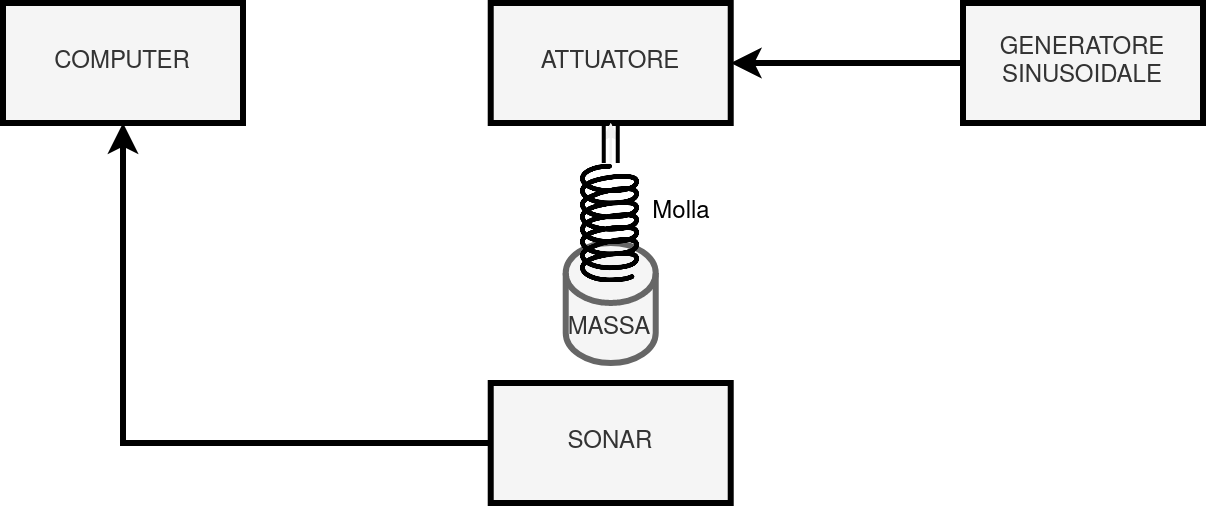
\includegraphics[width=0.8\textwidth]{diagramma.png}
  \captionsetup{labelformat=empty}
  \caption{Diagramma dell'apparato sperimentale.}
  \label{fig:diagramma.png}
\end{figure}

In appendice si trovano le foto della struttura e dell'attuatore.

% =================================================================================================

\section{Misure Effettuate}

Per l'esperimento, è stata scelta una configurazione massa-molla che si avvicinasse il più possibile al modello teorico. La massa è stata aumentata al fine di ottenere tempi di battimento più lunghi e per evitare che l'ampiezza della Lorentziana aumentasse eccessivamente.

Inizialmente, il sistema è stato messo in funzione e la pulsazione di risonanza approssimativa, $\omega_0$, è stata osservata. L'ampiezza della forzante è stata selezionata in modo da essere costante e abbastanza grande da consentire osservazioni delle oscillazioni fino a una distanza approssimativa di FWHM/2 dal centro, ma non così grande da far sì che le spire della molla raggiungessero la "battuta" durante la risonanza.

Per la raccolta dei dati, è stata scelta una frequenza della forzante, che è stata inserita nel generatore sinusoidale, e i dati sono stati poi acquisiti tramite il sonar. Utilizzando i dati raccolti, è stata effettuata una media dei massimi e una media dei minimi utilizzando il software CAPSTONE.

La stima sperimentale della frequenza di risonanza è stata ottenuta cercando direttamente dai dati la frequenza che massimizzava la risonanza. Successivamente, il valore è stato leggermente modificato per misurare più precisamente vicino alla frequenza di risonanza.

Sono state misurate le ampiezze di oscillazione per circa 10 frequenze, di cui almeno 5 all'interno dell'intervallo $\pm$FWHM/2 dal centro.

% =================================================================================================

\section{Analisi Dati}

Per l'analisi dei dati, è stato necessario calcolare l'ampiezza come differenza tra il valore massimo e il valore minimo dei dati raccolti. Successivamente, è stata propagata l'incertezza sui dati per ottenere un'incertezza associata all'ampiezza calcolata.

Per determinare la larghezza a metà altezza (FWHM), è stato calcolato il valore di metà altezza. Questo valore rappresenta il punto in cui l'ampiezza dell'oscillazione si dimezza rispetto al suo massimo. Il calcolo della FWHM è stato effettuato identificando i dati corrispondenti alla metà altezza e quelli al di fuori di essa. Attraverso l'interpolazione dei valori di soglia dagli estremi, è stata determinata la larghezza a metà altezza. L'incertezza della FWHM è stata affidata come il massimo del range di valori in cui può variare la vera FWHM in assenza di stime migliori.

Da questa FWHM, è stato calcolato il termine di smorzamento gamma utilizzando la formula:

\[ \gamma = \frac{\mathrm{{FWHM}}}{2\sqrt{3}} \]

Il termine di smorzamento gamma è una quantità che descrive l'ampiezza di attenuazione dell'oscillazione nel tempo.

Successivamente, è stata calcolata la Lorentziana attesa. Questo calcolo è stato effettuato sostituendo i valori noti, come $\omega_0$, $\omega_f$ e $\gamma$, nella formula della Lorentziana. 

\[ A(\omega_f)=\frac{F_0}{m\sqrt{\bigg(\omega_0^2-\omega_f^2\bigg)^2+4\gamma^2\omega_f^2}} \]

Si ottengono anche le incertezze sui valori $\sigma_L$ :

\[ \sigma_{L}=L^3f^2\gamma\sigma_{\gamma}^2 \]

Ottenere la Lorentziana attesa era importante per confrontare i dati sperimentali con i risultati previsti dalla teoria e valutare l'aderenza tra di essi. Per garantire una corretta comparazione tra i dati teorici e sperimentali, è stata eseguita la normalizzazione della Lorentziana teorica. Questo processo ha implicato l'imposizione di un coefficiente moltiplicativo tale che la somma delle misure teoriche fosse uguale alla somma delle misure sperimentali. La normalizzazione è stata eseguita al fine di consentire un confronto quantitativo diretto tra i due insiemi di dati.
Indichiamo con $D$ i valori sperimentali e $L$ i valori attesi, si impone quindi:

\[ \sum D=N\sum L \]

dove $N$ è il coefficiente di normalizzazione, di cui si trova anche l'incertezza $\sigma_N$ :

\[ \sigma_N=N\sqrt{\frac{\sum \sigma_L^2}{(\sum L)^2}+\frac{\sum \sigma_D^2}{(\sum D)^2}} \]

da cui si ricava l'incertezza sui valori attesi normalizzati $\sigma_{LN}$ :

\[
  \sigma_{LN}=LN\sqrt{\frac{\sigma_L^2}{L^2}+\frac{\sigma_N^2}{N^2}}
\]

I dati raccolti sono rappresentati nel grafico che segue.
\begin{figure}[htbp]
  \centering
  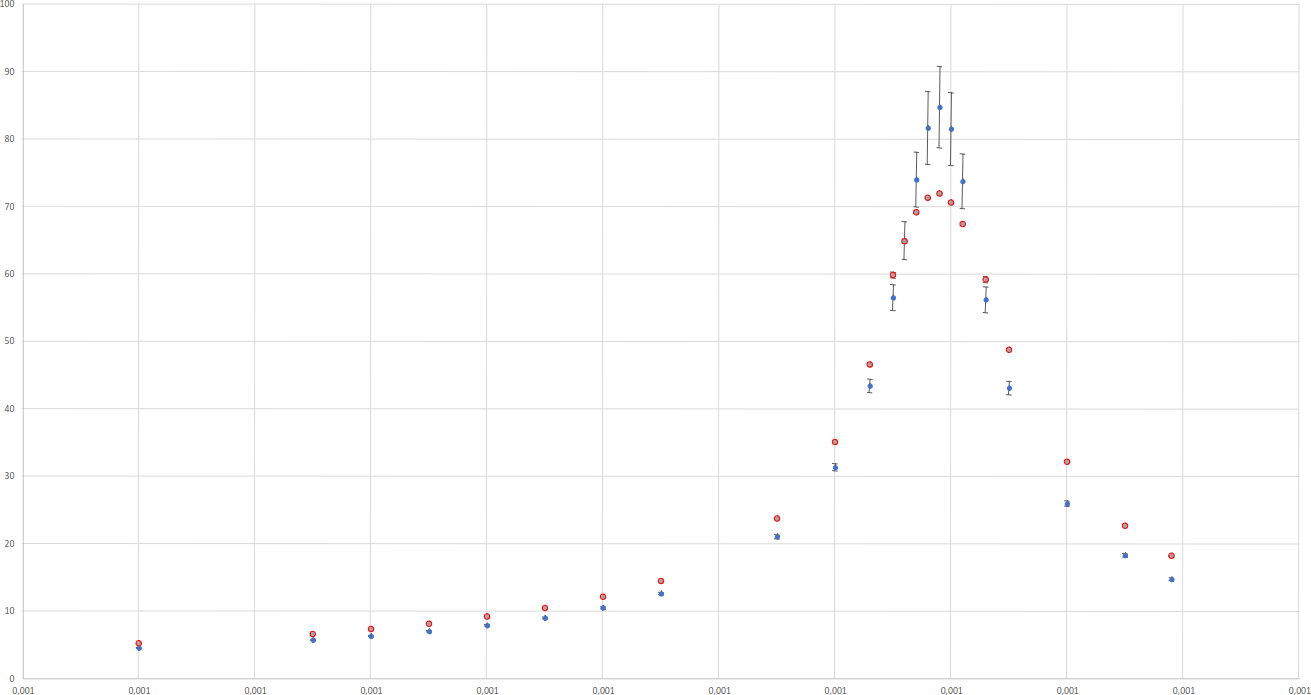
\includegraphics[width=1.0\textwidth]{grafico.png}
  \captionsetup{labelformat=empty}
  \caption{In rosso i valori attesi, in blu i valori sperimentali. Sulle ascisse la frequenza forzante (Hz), sulle ordinate l'ampiezza (mm).}
  \label{fig:grafico}
\end{figure}

Infine, per valutare la compatibilità tra la Lorentziana sperimentale e quella attesa, è stato eseguito un test del chi quadro. Le formule utilizzate per il test del chi quadro sono:

\[ \chi^2=\sum_{i=1}^{n}\frac{x_{i_{D}}^2+x_{i_{LN}}^2}{\sigma_i^2} \]
dove le incertezze sono:

\[ \sigma_i^2=\sigma_{i_{LN}}^2+\sigma_{i_{D}}^2 \]

L'esito del test del chi quadro è positivo, con una compatibilità fra curva sperimentale e teoria del 99,4\%.

% =================================================================================================

\section{Conclusione}

L'analisi dei dati raccolti durante l'esperimento ha confermato il valore stimato della frequenza di risonanza. Il valore ottenuto sperimentalmente per la frequenza di risonanza è risultato essere 1,049 $\pm$ 0,001 Hz.

Il confronto tra la curva di risonanza sperimentale e quella teorica ha mostrato un'elevata compatibilità. Il test del chi quadro ha confermato la compatibilità tra le due curve con una probabilità del 99,4\%.

Questi risultati confermano la validità del modello teorico utilizzato per descrivere il comportamento del sistema massa-molla smorzato e forzato. Tuttavia, è importante notare che il modello è un'approssimazione e non tiene conto di tutte le non idealità presenti nel sistema reale.

Inoltre, l'apparato e gli strumenti utilizzati per l'esperimento si sono dimostrati adeguati per la misura. Nonostante ciò, è possibile che miglioramenti specifici potrebbero ridurre ulteriormente le incertezze e migliorare la precisione dei risultati.

In conclusione, l'esperimento ha permesso di esaminare il fenomeno della risonanza in un sistema massa-molla smorzato e forzato, e di confrontare i risultati sperimentali con le previsioni teoriche.

\newpage

\section{Appendice}

\subsection{Dati dei Massimi e dei Minimi}

% ============================= inizio tabella =====================================

\begin{table}[ht]
  \begin{minipage}{0.40\textwidth}
    \centering
    \captionsetup{labelformat=empty} % Rimuove il numero della tabella
    \caption{Tabella 1: Dati dei Massimi}
    \begin{tabularx}{\linewidth}{|X|X|X|}
      \hline
      Frequenza (Hz) & Posizione (mm) & Errore (mm) \\
      \hline
      1,069 & 17,52 & 0,11 \\
      1,065 & 21,93 & 0,22 \\
      1,06 & 31,61 & 0,1 \\
      1,055 & 48,03 & 0,24 \\
      1,053 & 57,89 & 0,31 \\
      1,051 & 65,54 & 0,21 \\
      1,05 & 68,67 & 0,31 \\
      1,049 & 70,06 & 0,19 \\
      1,048 & 69,48 & 0,2 \\
      1,047 & 67,36 & 0,12 \\
      1,046 & 63,05 & 0,25 \\
      1,045 & 58,75 & 0,14 \\
      1,043 & 46,01 & 0,39 \\
      1,04 & 34,54 & 0,2 \\
      1,035 & 23,08 & 0,15 \\
      1,025 & 14,005 & 0,08625 \\
      1,02 & 11,73 & 0,07 \\
      1,015 & 10,07 & 0,11 \\
      1,01 & 8,88 & 0,1 \\
      1,005 & 7,73 & 0,00474 \\
      1 & 6,94 & 0,08 \\
      0,995 & 6,11 & 0,09 \\
      0,98 & 4,66 & 0,04 \\
      \hline
    \end{tabularx}
  \end{minipage}
  \hfill
  \begin{minipage}{0.40\textwidth}
    \centering
    \captionsetup{labelformat=empty} % Rimuove il numero della tabella
    \caption{Tabella 2: Dati dei Minimi}
    \begin{tabularx}{\linewidth}{|X|X|X|}
      \hline
      Frequenza (Hz) & Posizione (mm) & Errore (mm) \\
      \hline
      1,069 & -18,77 & 0,05 \\
      1,065 & -23,3 & 0,2 \\
      1,06 & -32,59 & 0,19 \\
      1,055 & -49,39 & 0,14 \\
      1,053 & -60,4 & 0,83 \\
      1,051 & -69,17 & 0,33 \\
      1,05 & -72,46 & 0,25 \\
      1,049 & -73,7 & 0,4 \\
      1,048 & -73,06 & 0,09 \\
      1,047 & -70,86 & 0,34 \\
      1,046 & -66,55 & 0,33 \\
      1,045 & -60,89 & 0,86 \\
      1,043 & -47,06 & 0,2 \\
      1,04 & -35,53 & 0,19 \\
      1,035 & -24,33 & 0,14 \\
      1,025 & -14,84 & 0,0764 \\
      1,02 & -12,42 & 0,07 \\
      1,015 & -10,75 & 0,09 \\
      1,01 & -9,43 & 0,12 \\
      1,005 & -8,462 & 0,00675 \\
      1 & -7,64 & 0,1 \\
      0,995 & -7,01 & 0,1 \\
      0,98 & -5,7 & 0,06 \\
      \hline
    \end{tabularx}
  \end{minipage}
\end{table}
  
  % ============================ fine tabella =========================================
\newpage

\subsection{Immagini}

\begin{figure}[htbp]
  \centering
  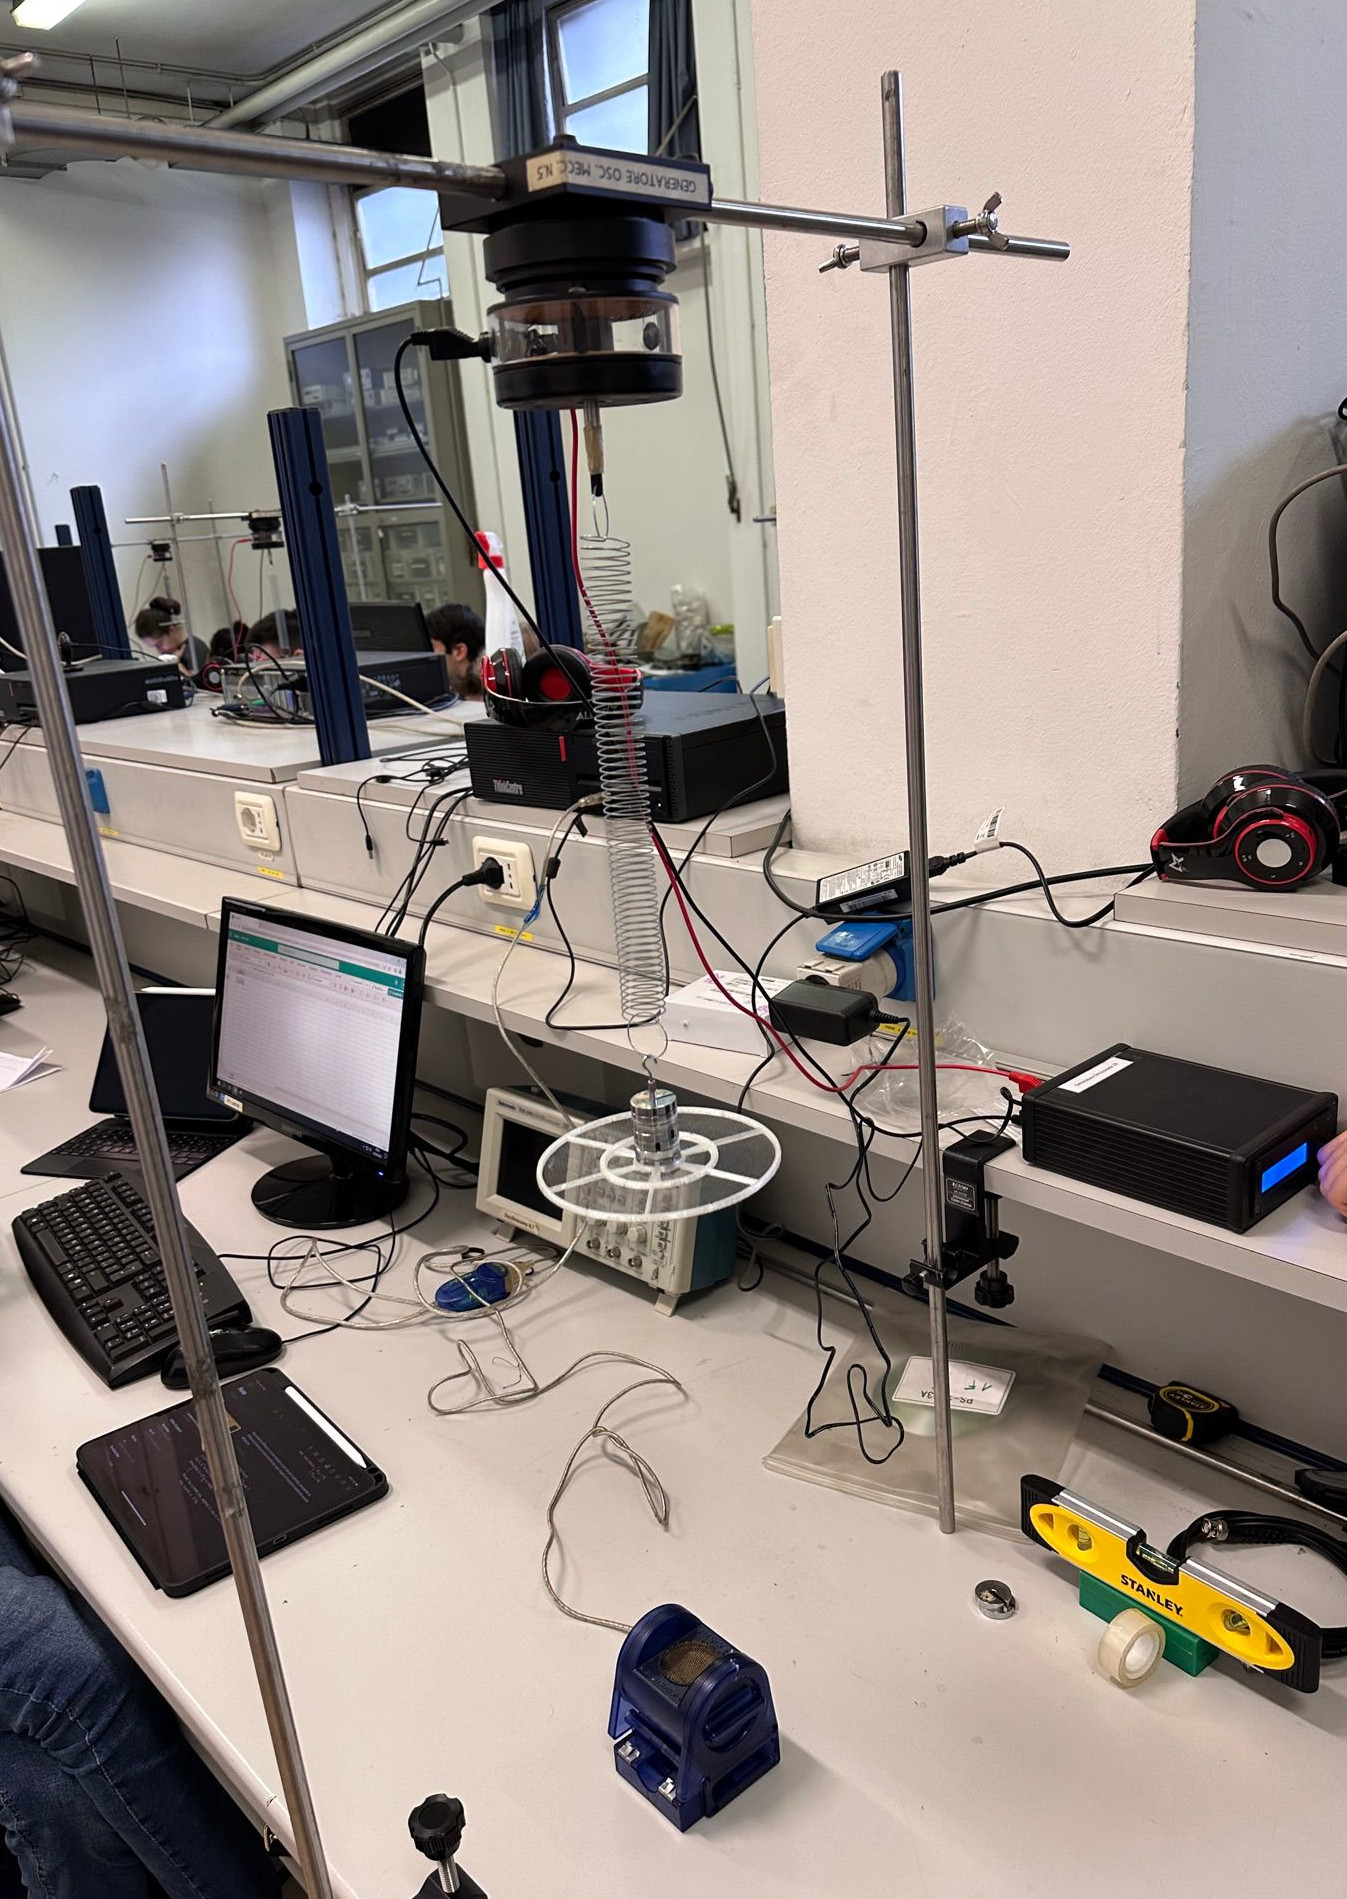
\includegraphics[width=0.75\textwidth]{struttura.jpeg}
  \captionsetup{labelformat=empty}
  \caption{Foto dell'apparato sperimentale: in basso il sonar collegato al computer, in alto l'attuatore a cui è appesa la molla, a destra il generatore sinusoidale.}
  \label{fig:struttura.jpeg}
\end{figure}

\begin{figure}[htbp]
  \centering
  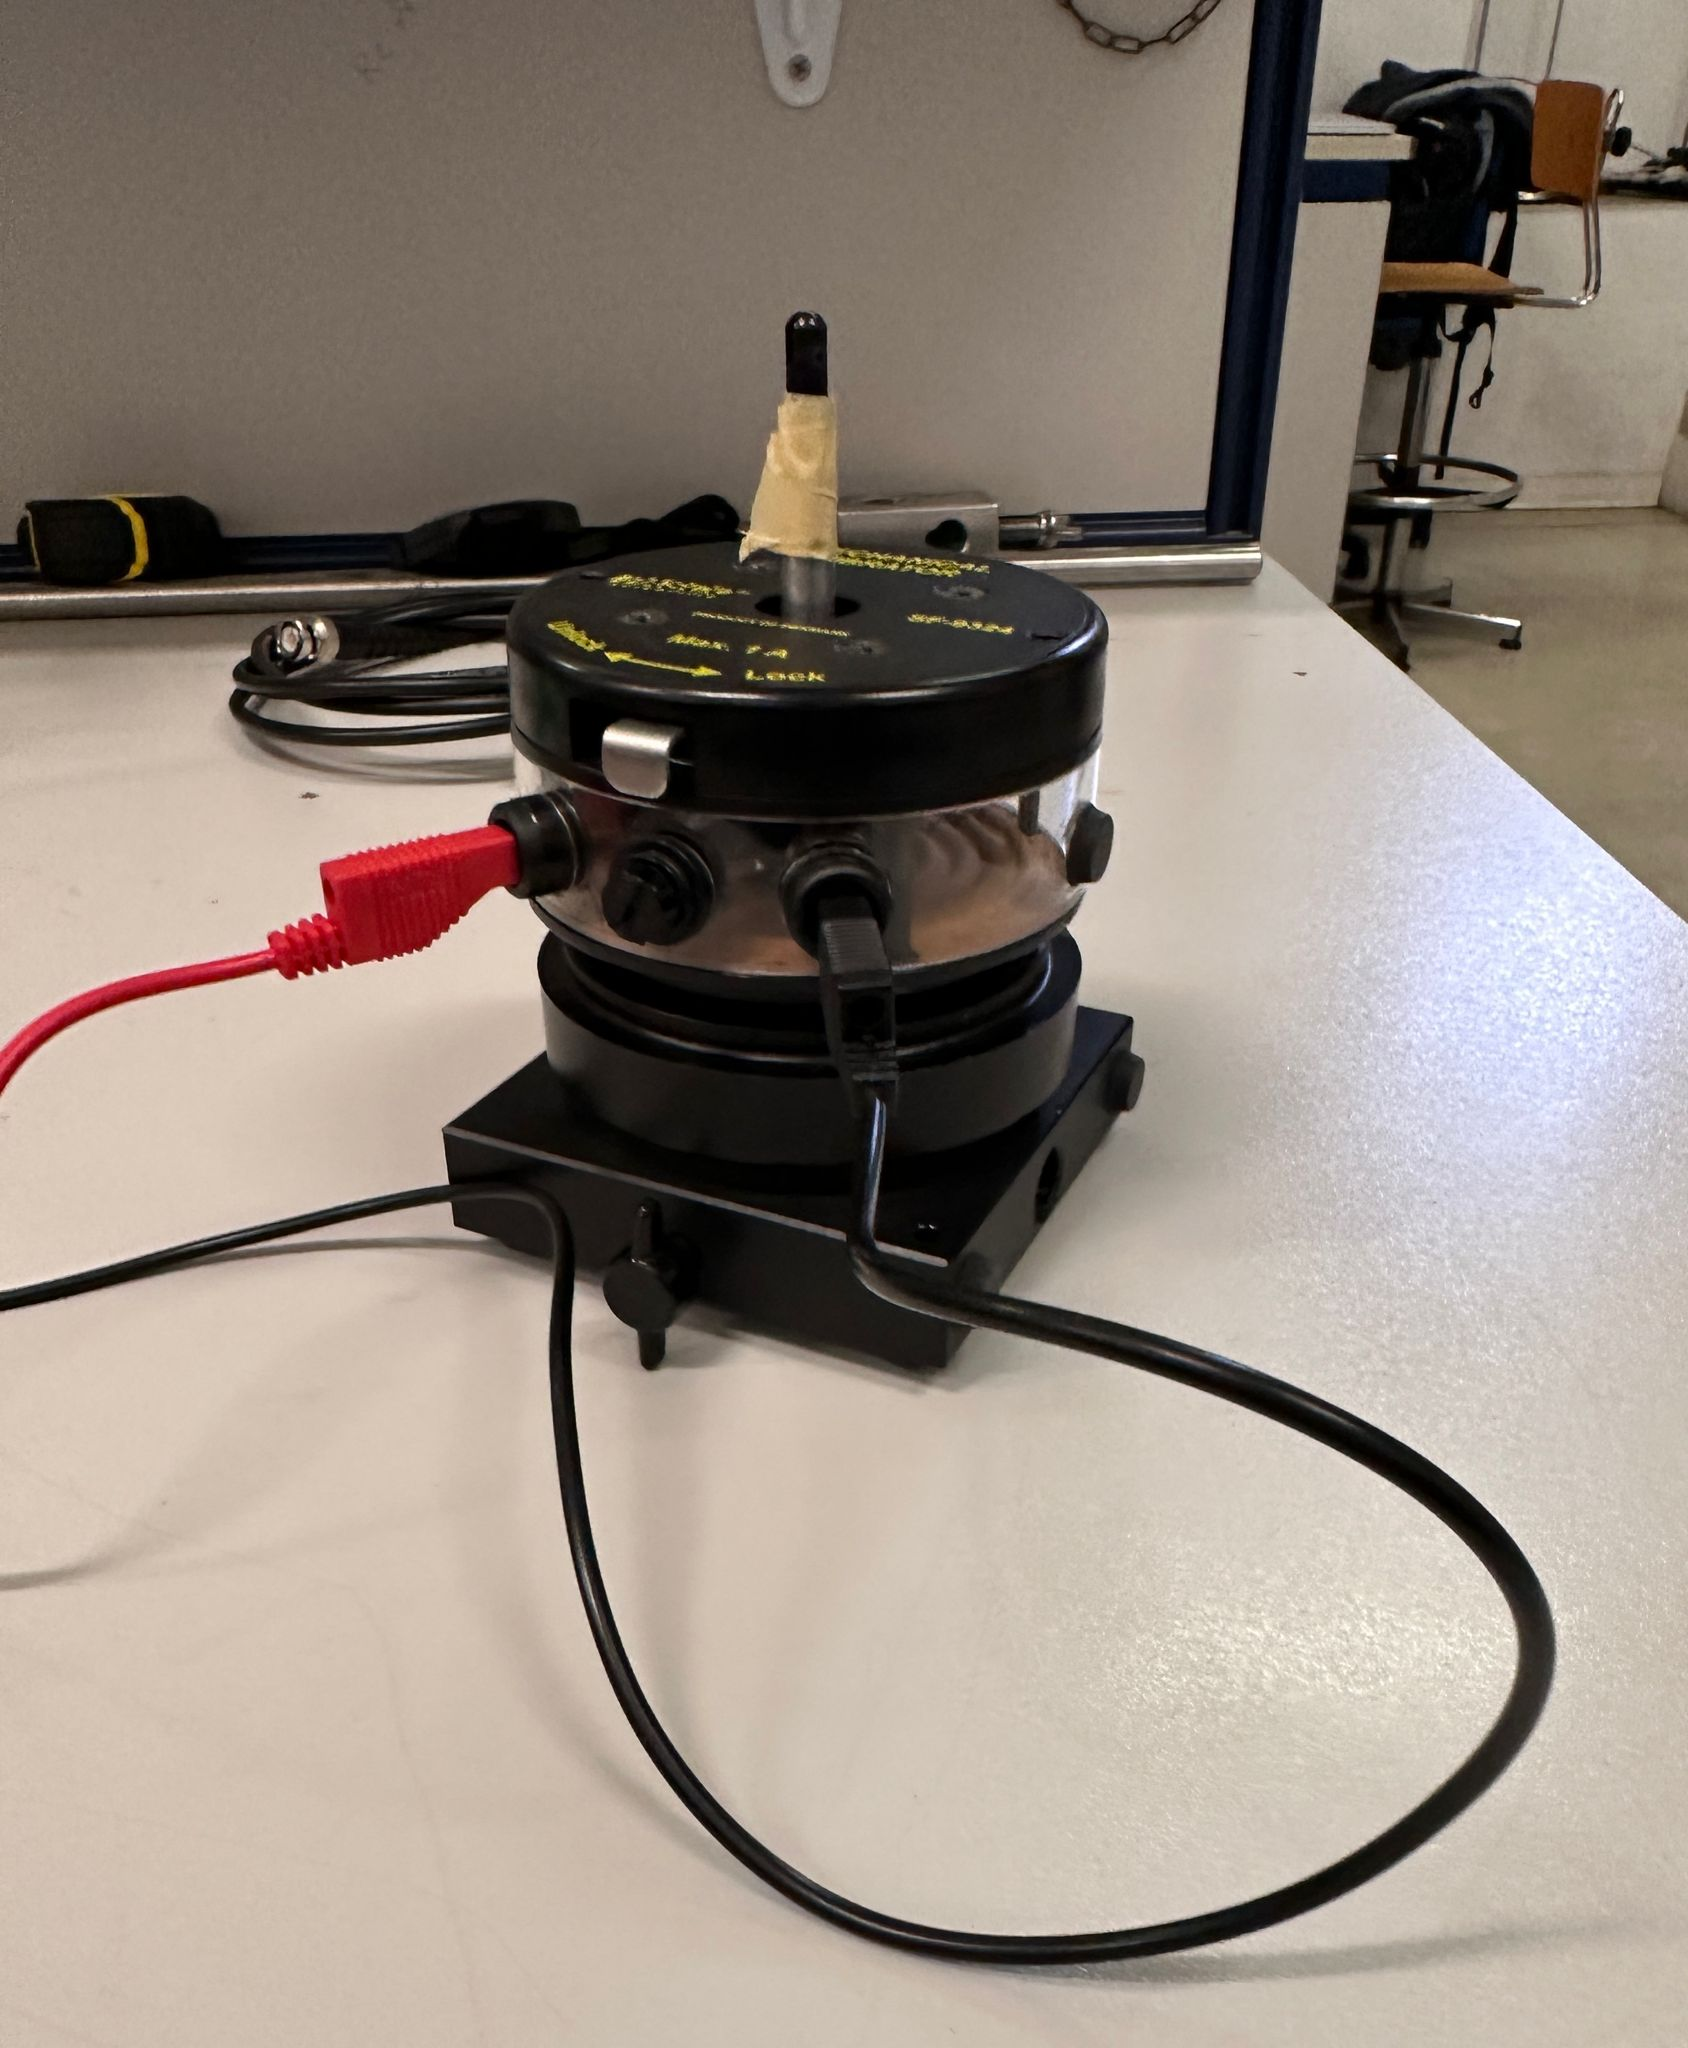
\includegraphics[width=0.75\textwidth]{attuatore.jpeg}
  \captionsetup{labelformat=empty}
  \caption{Foto dell'attuatore.}
  \label{fig:attuatore.jpeg}
\end{figure}

\end{document}
